%!TEX program = xelatex
%!TEX root = ../all_beamer.tex

% =========================================================
%  Foundations of Machine Learning — Chapter 3
%  Loss Functions & Training
%  Beamer presentation
% =========================================================
%% !TEX root = all_beamer.tex
% ==============================================================================
% HEADER LATEX PER PRESENTAZIONI BEAMER
% Corso di Machine Learning - Giorgio Gambosi
% Università di Roma "Tor Vergata"
% ==============================================================================

% ------------------------------------------------------------------------------
% CLASSE DOCUMENTO E METADATI
% ------------------------------------------------------------------------------
\documentclass[aspectratio=169, 10pt]{beamer}

\subtitle{Course of Machine Learning}
\author{Giorgio Gambosi}
\institute[Tor Vergata]{Master's Degree in Computer Science\\University of Rome ``Tor Vergata''}
\date{A.Y. 2025--2026}

% ------------------------------------------------------------------------------
% PACCHETTI MATEMATICI
% ------------------------------------------------------------------------------
\usepackage{amsmath, amssymb, amsfonts, mathtools, amsthm}
\usepackage{bm}              % Simboli matematici in grassetto
\usepackage{upgreek}         % Lettere greche dritte
\usepackage{derivative}      % Gestione semplificata delle derivate

% ------------------------------------------------------------------------------
% PACCHETTI GRAFICI E VISUALIZZAZIONE
% ------------------------------------------------------------------------------
\usepackage{graphicx}        % Inclusione immagini
\usepackage{xcolor}          % Gestione colori
\usepackage{xkcdcolors}      % Colori aggiuntivi stile xkcd
\usepackage{microtype}       % Miglioramenti tipografici

% ------------------------------------------------------------------------------
% PACCHETTI PER TABELLE
% ------------------------------------------------------------------------------
\usepackage{booktabs}        % Tabelle professionali
\usepackage{array}           % Estensioni per tabelle
\usepackage{multirow}        % Celle multi-riga
\usepackage{multicol}        % Layout multi-colonna

% ------------------------------------------------------------------------------
% TIKZ E PGFPLOTS
% ------------------------------------------------------------------------------
\usepackage{tikz}
\usepackage{tikz-network}
\usepackage[customcolors]{hf-tikz}
\usepackage{pgfplots}
\pgfplotsset{compat=1.18}
\usepgfplotslibrary{fillbetween}

% Librerie TikZ
\usetikzlibrary{arrows, arrows.meta, decorations.pathmorphing, decorations.pathreplacing}
\usetikzlibrary{decorations.markings, snakes, positioning, backgrounds, fit, shadows}
\usetikzlibrary{automata, patterns, calc, intersections, through, shapes}
\usetikzlibrary{shapes.geometric, shapes.arrows, scopes, chains, matrix}

% ------------------------------------------------------------------------------
% ALTRI PACCHETTI
% ------------------------------------------------------------------------------
\usepackage[skins]{tcolorbox}  % Box colorati
\usepackage{subcaption}         % Sottocaption per figure
\usepackage{listings}           % Inclusione codice sorgente

% ------------------------------------------------------------------------------
% TEMA E STILE BEAMER
% ------------------------------------------------------------------------------
\usetheme{Madrid}
\usecolortheme{whale}
\useinnertheme{rounded}
\usefonttheme{professionalfonts}
\setbeamertemplate{navigation symbols}{}  % Rimuove simboli di navigazione

% ------------------------------------------------------------------------------
% DEFINIZIONE COLORI PERSONALIZZATI
% ------------------------------------------------------------------------------
% Colori principali del tema
\definecolor{MainBlue}{RGB}{31,56,100}      % Blu principale (header, titoli)
\definecolor{AccentBlue}{RGB}{70,130,180}   % Blu accento (blocchi)
\definecolor{AlertRed}{RGB}{160,30,30}      % Rosso per alert
\definecolor{ExGreen}{RGB}{30,120,60}       % Verde per esempi
\definecolor{BlockBg}{RGB}{220,232,246}     % Sfondo blocchi
\definecolor{torgray}{RGB}{220,225,235}     % Grigio Tor Vergata

% Colori alternativi (Tor Vergata style)
\definecolor{TvDark}{RGB}{30,50,80}         % Blu scuro header
\definecolor{TvMid}{RGB}{70,100,140}        % Blu medio blocchi
\definecolor{TvLight}{RGB}{210,220,235}     % Blu chiaro sfondi
\definecolor{TvAlert}{RGB}{160,30,30}       % Rosso alert
\definecolor{TvGreen}{RGB}{20,100,50}       % Verde esempi

% Colori supplementari
\definecolor{torred}{RGB}{153,0,0}
\definecolor{torcyan}{RGB}{0,112,192}
\definecolor{cerise}{HTML}{DA3A62}
\definecolor{teal}{HTML}{029386}
\definecolor{slateblue}{HTML}{5B5EA6}
\definecolor{orange}{HTML}{F97306}

% Colori per nodi TikZ
\definecolor{nodeblue}{RGB}{101,140,196}    % xkcd Faded Blue

% ------------------------------------------------------------------------------
% CONFIGURAZIONE COLORI BEAMER
% ------------------------------------------------------------------------------
\setbeamercolor{frametitle}{bg=MainBlue, fg=white}
\setbeamercolor{title}{bg=MainBlue, fg=white}
\setbeamercolor{structure}{fg=MainBlue}

% Blocchi standard
\setbeamercolor{block title}{bg=AccentBlue, fg=white}
\setbeamercolor{block body}{bg=BlockBg}

% Blocchi alert
\setbeamercolor{block title alerted}{bg=AlertRed, fg=white}
\setbeamercolor{block body alerted}{bg=red!8}

% Blocchi esempio
\setbeamercolor{block title example}{bg=ExGreen, fg=white}
\setbeamercolor{block body example}{bg=green!7}

% ------------------------------------------------------------------------------
% CONFIGURAZIONE FONT BEAMER
% ------------------------------------------------------------------------------
\setbeamerfont{frametitle}{size=\normalsize,series=\bfseries}
\setbeamerfont{block title}{size=\small,series=\bfseries}

% ------------------------------------------------------------------------------
% STILI TIKZ PERSONALIZZATI
% ------------------------------------------------------------------------------
\tikzset{
  >=latex,  % Frecce stile LaTeX di default
  % Nodi per reti neurali
  node/.style={thick,circle,draw=myblue,minimum size=22,inner sep=0.5,outer sep=0.6},
  node in/.style={node,green!20!black,draw=mygreen!30!black,fill=mygreen!25},
  node hidden/.style={node,blue!20!black,draw=myblue!30!black,fill=myblue!20},
  node convol/.style={node,orange!20!black,draw=myorange!30!black,fill=myorange!20},
  node out/.style={node,red!20!black,draw=myred!30!black,fill=myred!20},
  % Connessioni
  connect/.style={thick,mydarkblue},
  connect arrow/.style={-{Latex[length=4,width=3.5]},thick,mydarkblue,shorten <=0.5,shorten >=1},
  % Stili numerati per facile mappatura
  node 1/.style={node in},
  node 2/.style={node hidden},
  node 3/.style={node out}
}

% ------------------------------------------------------------------------------
% AMBIENTI TEOREMI
% ------------------------------------------------------------------------------
\setbeamertemplate{theorems}[numbered]
\newtheorem{mytheorem}{Theorem}
\newtheorem{mydefinition}{Definition}

% ------------------------------------------------------------------------------
% CONFIGURAZIONE LISTINGS (CODICE)
% ------------------------------------------------------------------------------
\lstset{
  language=Python,
  basicstyle=\ttfamily\tiny,
  keywordstyle=\color{MainBlue}\bfseries,
  commentstyle=\color{gray},
  frame=single,
  breaklines=true,
}

% ==============================================================================
% MACRO MATEMATICHE PERSONALIZZATE
% ==============================================================================

% ------------------------------------------------------------------------------
% SPAZI CALLIGRAFICI (Calligraphic spaces)
% ------------------------------------------------------------------------------
\providecommand{\calX}{\mathcal{X}}         % Spazio input
\providecommand{\calY}{\mathcal{Y}}         % Spazio output
\providecommand{\calH}{\mathcal{H}}         % Spazio ipotesi
\providecommand{\calT}{\mathcal{T}}         % Training set
\providecommand{\calA}{\mathcal{A}}         % Algoritmo
\providecommand{\calR}{\mathcal{R}}         % Rischio
\providecommand{\calF}{\mathcal{F}}         % Famiglia di funzioni
\providecommand{\calL}{\mathcal{L}}         % Loss function

% Alias per compatibilità
\providecommand{\Rr}{\mathcal{R}}
\providecommand{\Tr}{\mathcal{T}}
\providecommand{\Hr}{\mathcal{H}}

% ------------------------------------------------------------------------------
% RISCHIO E PROBABILITÀ
% ------------------------------------------------------------------------------
\providecommand{\barR}{\overline{\mathcal{R}}}  % Rischio empirico
\providecommand{\EmpR}{\overline{\mathcal{R}}}  % Rischio empirico (alias)
\providecommand{\Rbar}{\overline{\mathcal{R}}}  % Rischio empirico (alias)
\providecommand{\pM}{p_M}                       % Probabilità modello
\providecommand{\pC}{p_C}                       % Probabilità corretta
\providecommand{\Prob}[2]{\mathbb{P}_{#1}\!\left[#2\right]}  % Probabilità

% ------------------------------------------------------------------------------
% FUNZIONI INDICATRICI
% ------------------------------------------------------------------------------
\providecommand{\indicator}[1]{\mathbf{1}\!\left[#1\right]}  % Funzione indicatrice
\providecommand{\ind}[1]{\mathbf{1}[#1]}                      % Versione breve

% ------------------------------------------------------------------------------
% OPERATORI MATEMATICI
% ------------------------------------------------------------------------------
\providecommand{\argmax}{\operatorname*{arg\,max}}  % Argomento del massimo
\providecommand{\argmin}{\operatorname*{arg\,min}}  % Argomento del minimo
\providecommand{\vcd}[1]{\operatorname{VCdim}(#1)} % VC dimension
\providecommand{\defeq}{\stackrel{\text{def}}{=}}  % Definito come

% ------------------------------------------------------------------------------
% VETTORI E MATRICI (Bold Math)
% ------------------------------------------------------------------------------
% Vettori minuscoli
\providecommand{\bx}{\mathbf{x}}            % Vettore x
\providecommand{\bz}{\mathbf{z}}            % Vettore z
\providecommand{\bw}{\mathbf{w}}            % Vettore peso
\providecommand{\btt}{\mathbf{t}}           % Vettore target
\providecommand{\wvec}{\mathbf{w}}          % Vettore peso (alias)
\providecommand{\bth}{\boldsymbol{\theta}}  % Parametro theta

% Matrici maiuscole
\providecommand{\bX}{\mathbf{X}}            % Matrice dati
\providecommand{\bZ}{\mathbf{Z}}            % Matrice Z
\providecommand{\Xmat}{\mathbf{X}}          % Matrice dati (alias)
\providecommand{\Hmat}{\mathbf{H}}          % Matrice H
\providecommand{\Smat}{\mathbf{S}}          % Matrice scatter generica
\providecommand{\bS}{\mathbf{S}}            % Matrice scatter
\providecommand{\Ii}{\mathbf{I}}            % Matrice identità
\providecommand{\bZero}{\mathbf{0}}         % Vettore zero
\providecommand{\bPsi}{\boldsymbol{\Psi}}   % Matrice Psi

% Medie (overline)
\providecommand{\ox}{\overline{\mathbf{x}}} % Media vettore x
\providecommand{\ow}{\overline{\mathbf{w}}} % Media vettore w
\providecommand{\oX}{\overline{\mathbf{X}}} % Media matrice X

% Matrici scatter specifiche (analisi discriminante)
\providecommand{\SW}{\mathbf{S}_W}          % Within-class scatter
\providecommand{\SB}{\mathbf{S}_B}          % Between-class scatter
\providecommand{\ST}{\mathbf{S}_T}          % Total scatter
\providecommand{\GX}{G_{\mathbf{X}}}        % Matrice Gram

% ------------------------------------------------------------------------------
% COMANDI DI FORMATTAZIONE TESTO
% ------------------------------------------------------------------------------
\providecommand{\term}[1]{\textbf{\color{accent}#1}}        % Termine importante
\providecommand{\halert}[1]{{\color{AlertRed}\textbf{#1}}}  % Alert rosso
\providecommand{\mlalert}[1]{{\color{AccentBlue}\textbf{#1}}}  % Alert blu
\providecommand{\mlemph}[1]{{\color{MainBlue}\textit{#1}}}  % Enfasi blu

% ==============================================================================
% FINE HEADER
% ==============================================================================

\newcommand{\blankpage}{
\clearpage
\thispagestyle{empty}
\null
\clearpage
}


%\documentclass[aspectratio=169,10pt]{beamer}
%
%% ---------- Theme & colours ----------
%\usetheme{Madrid}
%\usecolortheme{whale}
%%\useoutertheme{miniframes}
%\useinnertheme{rounded}
%\setbeamertemplate{navigation symbols}{}
%
%\definecolor{MainBlue}{RGB}{31,56,100}
%\definecolor{AccentBlue}{RGB}{70,130,180}
%\definecolor{AlertRed}{RGB}{160,30,30}
%\definecolor{ExGreen}{RGB}{30,120,60}
%\definecolor{BlockBg}{RGB}{220,232,246}
%\definecolor{torgray}{RGB}{220,225,235}
%
%%\definecolor{MainBlue}{RGB}{0,62,126}
%%\definecolor{TorVergataGold}{RGB}{200,150,0}
%%\definecolor{AlertRed}{RGB}{180,30,30}
%%\definecolor{ExampleGreen}{RGB}{20,120,60}
%%\definecolor{LightBlue}{RGB}{220,235,250}
%%\definecolor{LightGreen}{RGB}{220,245,230}
%%\definecolor{LightRed}{RGB}{250,225,225}
%
%\setbeamercolor{frametitle}{bg=MainBlue, fg=white}
%\setbeamercolor{title}{bg=MainBlue, fg=white}
%\setbeamercolor{block title}{bg=AccentBlue, fg=white}
%\setbeamercolor{block body}{bg=BlockBg}
%\setbeamercolor{block title alerted}{bg=AlertRed, fg=white}
%\setbeamercolor{block body alerted}{bg=red!8}
%\setbeamercolor{block title example}{bg=ExGreen, fg=white}
%\setbeamercolor{block body example}{bg=green!7}
%\setbeamercolor{structure}{fg=MainBlue}
%
%%\setbeamercolor{frametitle}{bg=MainBlue,fg=white}
%%\setbeamercolor{title}{bg=MainBlue,fg=white}
%%\setbeamercolor{structure}{fg=MainBlue}
%%\setbeamercolor{block title}{bg=MainBlue,fg=white}
%%\setbeamercolor{block body}{bg=LightBlue}
%%\setbeamercolor{block title alerted}{bg=AlertRed,fg=white}
%%\setbeamercolor{block body alerted}{bg=LightRed}
%%\setbeamercolor{block title example}{bg=ExampleGreen,fg=white}
%%\setbeamercolor{block body example}{bg=LightGreen}

% ---------- Packages ----------
%\usepackage{amsmath,amssymb,mathtools}
%\usepackage{booktabs}
%\usepackage{graphicx}
%\usepackage{xcolor}
%\usepackage{tikz}
%\usetikzlibrary{arrows.meta,positioning}
%\usepackage{listings}
%\usepackage{array}
%\usepackage{multirow}
%
%\lstset{
%  language=Python,
%  basicstyle=\ttfamily\tiny,
%  keywordstyle=\color{MainBlue}\bfseries,
%  commentstyle=\color{gray},
%  frame=single,
%  breaklines=true,
%}
%
%% ---------- Macros ----------
%\newcommand{\bth}{\boldsymbol{\theta}}
%\newcommand{\bx}{\mathbf{x}}
%\newcommand{\bw}{\mathbf{w}}
%\newcommand{\calT}{\mathcal{T}}
%\newcommand{\calL}{\mathcal{L}}
%\newcommand{\Rbar}{\overline{\mathcal{R}}}
%\newcommand{\defeq}{\stackrel{\text{def}}{=}}

\title[Loss Function Optimization]{Loss Function Optimization}
%\subtitle{Course of Machine Learning}
%\author{Giorgio Gambosi}
%\institute{Master's Degree in Computer Science\\University of Rome ``Tor Vergata''}
%\date{A.Y.\ 2025–2026}
% ---------- Meta ----------

% =========================================================
%\begin{document}

\begin{frame}[plain]
  \titlepage
\end{frame}

% ----- Outline -----
\begin{frame}{Outline}
  \tableofcontents
\end{frame}

% =========================================================
\section{Loss Functions}
% =========================================================

\begin{frame}{The Loss Function — Concept}
  \begin{block}{Definition}
    The \textbf{loss function} $\mathcal{L}:\mathcal{Y}\times\mathcal{Y}\to\Real$
    measures the \textcolor{AlertRed}{cost} of predicting $y$ when the true target is $t$.
  \end{block}
  \vspace{6pt}
  \begin{itemize}
    \item Both $y$ (prediction) and $t$ (target) belong to the output space $\mathcal{Y}$.
    \item $\mathcal{Y}$ can be: real numbers (regression), class labels (classification), structured outputs.
    \item For a single input $\bx$ with true output $t$, the pointwise quality is:
      \[
        \mathcal{R}(\bx,t) = L(h(\bx),\,t)
      \]
    \item The loss function drives the \emph{definition} of what ``good predictions'' means.
  \end{itemize}
\end{frame}

% ----- Empirical Risk -----
\begin{frame}{Empirical Risk}
  \begin{block}{Definition}
    The \textbf{empirical risk} aggregates the loss over the training set $\calT$:
    \[
      \Rbar_{\calT}(h)
      = \frac{1}{|\calT|}\sum_{(\bx,t)\in\calT} L(h(\bx),t)
    \]
  \end{block}
  \vspace{6pt}
  \begin{itemize}
    \item Measures the \emph{average} error of $h$ on the available data.
    \item Lower value $\Rightarrow$ better fit to training data.
    \item \textcolor{AlertRed}{Caveat:} minimising empirical risk $\neq$ minimising generalisation error.
    \item True goal: perform well on \emph{unseen} data (generalisation).
  \end{itemize}
\end{frame}

% ----- Parametric Models -----
\begin{frame}{Parametric Models \& Overall Loss}
  \begin{itemize}
    \item In practice, $h = h_{\bth}$ where $\bth = (\theta_0,\ldots,\theta_d)$ are learned parameters.
    \item Training $=$ searching for the $\bth$ minimising:
      \[
        \calL(\bth;\calT) = \sum_{i=1}^n L_i(\bth)
        \quad\text{where}\quad
        L_i = L(\bth;\bx_i,t_i)
      \]
    \item The overall loss sums individual contributions from each example.
  \end{itemize}
  \begin{exampleblock}{Interpretation}
    Each data point $(\bx_i,t_i)$ contributes a term $L_i(\bth)$ that penalises the model for
    predicting incorrectly on that specific example.
    Training adjusts $\bth$ to reduce this total penalty.
  \end{exampleblock}
\end{frame}

% =========================================================
\section{Optimisation of the Loss}
% =========================================================

\begin{frame}{Goal: Finding a Global Minimum}
  \begin{itemize}
    \item We seek a \textcolor{MainBlue}{global minimum} of $\calL(\bth;\calT)$
          over the parameter space.
    \item A global minimum is a point where the loss is \emph{lower than at every other point}.
  \end{itemize}
  \begin{block}{Calculus Approach}
    At any minimum (local or global), the gradient must vanish:
    \[
      \nabla\calL(\bth;\calT) = \Zero
      \qquad\Longleftrightarrow\qquad
      \frac{\partial}{\partial\theta_i}\calL(\bth;\calT) = 0
      \quad\forall i
    \]
  \end{block}
  \begin{itemize}
    \item \textbf{Gradient} $\nabla f$ at a point: vector of steepest ascent.
    \item \textbf{Negative gradient} $-\nabla f$: direction of steepest descent.
  \end{itemize}
\end{frame}

% ----- Challenges -----
\begin{frame}{Challenges of Analytical Solutions}
  Setting $\nabla\calL = \Zero$ has several \textcolor{AlertRed}{critical limitations}:
  \begin{itemize}
    \item \textbf{Multiple solutions}: critical points include minima, maxima, \emph{and} saddle points.
    \item \textbf{Analytical intractability}: complex models (e.g.\ neural networks)
          rarely admit closed-form solutions.
    \item \textbf{Non-linearity}: deep networks compose many non-linear functions —
          no algebraic formula exists.
  \end{itemize}
  \begin{alertblock}{Consequence}
    In most practical settings we must resort to \textbf{iterative numerical methods}.
  \end{alertblock}
\end{frame}

% =========================================================
\section{Gradient Descent}
% =========================================================

\begin{frame}{Gradient Descent — Principle}
  \begin{block}{Core idea}
    Move iteratively in the direction of \textcolor{AlertRed}{steepest descent}
    of the empirical risk.
  \end{block}
  \vspace{6pt}
  \begin{itemize}
    \item Initialise parameters:
          $\bth^{(0)} = (\theta_0^{(0)},\ldots,\theta_d^{(0)})$ (often random).
    \item At each iteration $i$, update \emph{every} parameter:
      \[
        \theta_j^{(i)}
        \;\leftarrow\;
        \theta_j^{(i-1)}
        - \eta\,
        \frac{\partial}{\partial\theta_j}
        \Rbar_{\calT}(\bth)\Big|_{\bth^{(i-1)}}
      \]
    \item $\eta > 0$ is the \textbf{learning rate}: controls the step size.
  \end{itemize}
\end{frame}

% ----- Matrix Form -----
\begin{frame}{Gradient Descent — Matrix Form}
  In compact matrix notation, the update becomes:
  \[
    \bth^{(i)}
    \;\leftarrow\;
    \bth^{(i-1)}
    - \frac{\eta}{|\calT|}
    \sum_{(\bx,t)\in\calT}
    \nabla L(h_{\bth}(\bx),t)\Big|_{\bth^{(i-1)}}
  \]
  \begin{itemize}
    \item All parameters are updated \emph{simultaneously}.
    \item The gradient is evaluated on the \emph{entire} training set at each step.
    \item This variant is called \textbf{batch gradient descent}.
  \end{itemize}
  \begin{exampleblock}{Intuition}
    Think of a ball rolling down a landscape: at each step it moves in the direction
    the slope is steepest, eventually settling in a valley.
  \end{exampleblock}
\end{frame}

% ----- Batch GD figures -----
\begin{frame}{Batch Gradient Descent — Behavior}
  \begin{columns}
    \column{0.5\textwidth}
      \begin{figure}
        \centering
        
\includegraphics[width=\linewidth]{figures/batchgd0.png}
        \caption{Cost vs.\ number of iterations}
      \end{figure}
    \column{0.5\textwidth}
      \begin{figure}
        \centering
        
\includegraphics[width=\linewidth]{figures/batchgd1.png}
        \caption{Trajectory in feature space}
      \end{figure}
  \end{columns}
  \vspace{4pt}
  \centering\small Batch gradient descent behavior
\end{frame}

% ----- Learning Rate -----
\begin{frame}{The Learning Rate $\eta$}
  \begin{columns}[t]
    \column{0.45\textwidth}
      \begin{block}{Too small $\eta$}
        \begin{itemize}
          \item Very slow convergence.
          \item Reliable but impractical for large models.
        \end{itemize}
      \end{block}
      \vspace{6pt}
      \begin{alertblock}{Too large $\eta$}
        \begin{itemize}
          \item May overshoot the minimum.
          \item Can oscillate or diverge.
        \end{itemize}
      \end{alertblock}
    \column{0.52\textwidth}
      \begin{block}{Challenges in practice}
        \begin{itemize}
          \item Many local minima in non-convex landscapes.
          \item Saddle points: gradient $= \Zero$, yet not a minimum.
          \item Convergence speed depends on curvature and $\eta$.
          \item Modern solutions: momentum, adaptive rates (Adam, RMSProp).
        \end{itemize}
      \end{block}
  \end{columns}
\end{frame}

% ----- Batch GD — Linear Regression -----
\begin{frame}{Batch GD — Linear Regression Update}
  For $h(\bx) = \sum_s \theta_s x_s + \theta_0$, the update rules are:
  \begin{align*}
    \theta_j^{(k+1)} &= \theta_j^{(k)}
      - \frac{\eta}{|\calT|}
      \sum_{(\bx,t)\in\calT}
      \!\!\left(\sum_{s=1}^d\theta_s^{(k)}x_s+\theta_0^{(k)}-t\right)x_j,
      \quad j=1,\ldots,d\\[6pt]
    \theta_0^{(k+1)} &= \theta_0^{(k)}
      - \frac{\eta}{|\calT|}
      \sum_{(\bx,t)\in\calT}
      \!\!\left(\sum_{s=1}^d\theta_s^{(k)}x_s+\theta_0^{(k)}-t\right)
  \end{align*}
  \begin{itemize}
    \item Gradients are \emph{linear} in the parameters.
    \item Setting to zero yields the \textbf{normal equations} (closed-form solution).
    \item Batch GD is \textbf{guaranteed to converge} to the global minimum for convex losses.
  \end{itemize}
\end{frame}

% =========================================================
\section{Stochastic Gradient Descent}
% =========================================================

\begin{frame}{Stochastic Gradient Descent (SGD)}
  \begin{block}{Motivation}
    Batch GD computes the gradient over the \emph{entire} training set at each step.
    This is expensive when $|\calT|$ is large.
  \end{block}
  \vspace{6pt}
  \begin{block}{SGD idea}
    Use a \textcolor{AlertRed}{single randomly chosen} example $(\bx_i,t_i)$
    to estimate the gradient:
    \[
      \bth^{(i)}
      \;\leftarrow\;
      \bth^{(i-1)}
      - \eta\,\nabla L(h_{\bth}(\bx_i),t_i)\Big|_{\bth^{(i-1)}}
    \]
  \end{block}
  \begin{itemize}
    \item Noisy gradient estimate, but very fast per step.
    \item Noise can \emph{help} escape local minima.
    \item Widely used in deep learning practice.
  \end{itemize}
\end{frame}

% ----- SGD figures -----
\begin{frame}{SGD — Behavior}
  \begin{columns}
    \column{0.5\textwidth}
      \begin{figure}
        \centering
        
\includegraphics[width=\linewidth]{figures/sgd0.png}
        \caption{Cost vs.\ number of iterations}
      \end{figure}
    \column{0.5\textwidth}
      \begin{figure}
        \centering
        
\includegraphics[width=\linewidth]{figures/sgd1.png}
        \caption{Trajectory in feature space}
      \end{figure}
  \end{columns}
  \vspace{4pt}
  \centering\small Stochastic gradient descent behavior
\end{frame}

% ----- Mini-batch -----
\begin{frame}{Mini-Batch Gradient Descent}
  \begin{block}{Compromise}
    Use a \textbf{mini-batch} $B\subset\calT$ of $m$ randomly chosen examples:
    \[
      \bth^{(i)}
      \;\leftarrow\;
      \bth^{(i-1)}
      - \frac{\eta}{m}
      \sum_{(\bx,t)\in B}
      \nabla L(h_{\bth}(\bx),t)\Big|_{\bth^{(i-1)}}
    \]
  \end{block}
  \vspace{4pt}
  \begin{center}
  \renewcommand{\arraystretch}{1.3}
  \begin{tabular}{lccc}
    \toprule
     & \textbf{Batch} & \textbf{Mini-batch} & \textbf{SGD}\\
    \midrule
    Gradient quality & exact & good estimate & noisy\\
    Speed per step   & slow  & moderate       & fast\\
    Memory use       & full  & moderate       & minimal\\
    Typical use      & small $n$ & deep learning & large $n$\\
    \bottomrule
  \end{tabular}
  \end{center}
\end{frame}

% ----- Mini-batch figures -----
\begin{frame}{Mini-Batch GD — Behavior}
  \begin{columns}
    \column{0.5\textwidth}
      \begin{figure}
        \centering
        
\includegraphics[width=\linewidth]{figures/mbgd0.png}
        \caption{Cost vs.\ number of iterations}
      \end{figure}
    \column{0.5\textwidth}
      \begin{figure}
        \centering
        
\includegraphics[width=\linewidth]{figures/mbgd1.png}
        \caption{Trajectory in feature space}
      \end{figure}
  \end{columns}
  \vspace{4pt}
  \centering\small Mini-batch gradient descent behavior
\end{frame}

% ----- Open issues -----
\begin{frame}{Open Issues with Basic GD Variants}
  \begin{itemize}
    \item \textbf{Learning rate selection}: too small $\Rightarrow$ slow; too large $\Rightarrow$ diverge.
    \item \textbf{Learning rate schedules} help but require problem-specific hyperparameters.
    \item \textbf{Single global rate}: suboptimal when features have different scales or frequencies.
    \item \textbf{Non-convex landscapes}: many local minima and saddle points;
          flat regions where gradients $\approx\Zero$ in all directions.
  \end{itemize}
  \begin{alertblock}{Motivation for advanced optimisers}
    These issues motivate momentum methods and adaptive learning-rate algorithms.
  \end{alertblock}
\end{frame}

% =========================================================
\section{Momentum \& Adaptive Methods}
% =========================================================

\begin{frame}{Momentum Gradient Descent — Principle}
  \begin{block}{Physical analogy}
    Parameters $\bth$ model the position of a unit-mass body sliding over the cost surface.
    The negative gradient $-\eta\nabla J$ acts as a force (acceleration).
  \end{block}
  \vspace{6pt}
  \begin{itemize}
    \item Standard GD resets velocity at each step — no memory of past motion.
    \item \textbf{Momentum GD} adds a velocity term:
      \begin{align*}
        v_j^{(k+1)} &= \gamma\, v_j^{(k)} - \eta\, g_{j,k}\\
        \theta_j^{(k+1)} &= \theta_j^{(k)} + v_j^{(k+1)}
      \end{align*}
    \item $\gamma\in[0,1)$ is the \emph{momentum coefficient} (friction parameter).
    \item Updates are a \emph{damped sum of all past gradients}.
  \end{itemize}
\end{frame}

% ----- Momentum figures -----
\begin{frame}{Momentum — Effect on Trajectory}
  \begin{columns}
    \column{0.5\textwidth}
      \begin{figure}
        \centering
        
\includegraphics[width=\linewidth]{figures/no_momentum.png}
        \caption{GD without momentum}
      \end{figure}
    \column{0.5\textwidth}
      \begin{figure}
        \centering
        
\includegraphics[width=\linewidth]{figures/momentum.png}
        \caption{Momentum GD}
      \end{figure}
  \end{columns}
  \vspace{4pt}
  \centering\small Momentum effect on trajectory
\end{frame}

\begin{frame}{Momentum GD — Behavior}
  \begin{columns}
    \column{0.5\textwidth}
      \begin{figure}
        \centering
        
\includegraphics[width=\linewidth]{figures/mgd0.png}
        \caption{Cost vs.\ number of iterations}
      \end{figure}
    \column{0.5\textwidth}
      \begin{figure}
        \centering
        
\includegraphics[width=\linewidth]{figures/mgd1.png}
        \caption{Trajectory in feature space}
      \end{figure}
  \end{columns}
  \vspace{4pt}
  \centering\small Momentum gradient descent behavior
\end{frame}

% ----- Nesterov -----
\begin{frame}{Nesterov Accelerated Gradient (NAG)}
  \begin{block}{Key idea}
    Evaluate the gradient at a \emph{look-ahead} position rather than the current one.
  \end{block}
  \vspace{6pt}
  \begin{itemize}
    \item Look-ahead estimate:
      $\tilde{\bth}^{(k+1)} \defeq \bth^{(k)} + \gamma v^{(k)}$
    \item NAG update:
      \begin{align*}
        \tilde\theta_j^{(k+1)} &= \theta_j^{(k)} + \gamma v_j^{(k)}\\
        v_j^{(k+1)} &= \gamma v_j^{(k)} - \eta\, g_{j,k+1}\\
        \theta_j^{(k+1)} &= \tilde\theta_j^{(k)} + v_j^{(k+1)}
      \end{align*}
    \item Anticipates changes in velocity — corrects trajectory \emph{earlier}.
    \item Results in more responsive and often faster convergence than plain momentum.
  \end{itemize}
\end{frame}

% ----- NAG figures -----
\begin{frame}{Nesterov vs.\ Momentum — Step Comparison}
  \begin{center}
    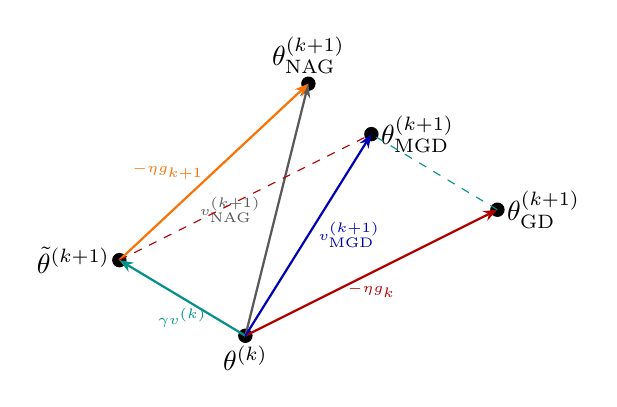
\begin{tikzpicture}[scale=1.6,
      arr/.style={-{Stealth[length=5pt]},thick}]
      \coordinate (A) at (0,0);
      \coordinate (C) at (-1,.6);
      \coordinate (D) at (2,1);
      \coordinate (E) at (0.5,2);
      \coordinate (B) at (1,1.6);
      \draw[fill=black] (A) circle (1.5pt) node[below]{$\theta^{(k)}$};
      \draw[fill=black] (E) circle (1.5pt) node[above]{$\theta^{(k+1)}_{\mathrm{NAG}}$};
      \draw[fill=black] (C) circle (1.5pt) node[left]{$\tilde\theta^{(k+1)}$};
      \draw[fill=black] (B) circle (1.5pt) node[right]{$\theta^{(k+1)}_{\mathrm{MGD}}$};
      \draw[fill=black] (D) circle (1.5pt) node[right]{$\theta^{(k+1)}_{\mathrm{GD}}$};
      \draw[arr,gray!70!black] (A)--(E) node[midway,left,xshift=-2pt,font=\tiny]{$v^{(k+1)}_{\mathrm{NAG}}$};
      \draw[arr,teal] (A)--(C) node[midway,below,font=\tiny]{$\gamma v^{(k)}$};
      \draw[arr,orange] (C)--(E) node[midway,left,font=\tiny]{$-\eta g_{k+1}$};
      \draw[arr,red!70!black] (A)--(D) node[midway,below,font=\tiny]{$-\eta g_k$};
      \draw[arr,blue!70!black] (A)--(B) node[midway,right,font=\tiny]{$v^{(k+1)}_{\mathrm{MGD}}$};
      \draw[red!70!black,dashed,thin](C)--(B);
      \draw[teal,dashed,thin](D)--(B);
    \end{tikzpicture}
  \end{center}
  \small Nesterov vs.\ momentum GD vs.\ GD steps
\end{frame}

\begin{frame}{NAG — Behavior}
  \begin{columns}
    \column{0.5\textwidth}
      \begin{figure}
        \centering
        
\includegraphics[width=\linewidth]{figures/ngd0.png}
        \caption{Cost vs.\ number of iterations}
      \end{figure}
    \column{0.5\textwidth}
      \begin{figure}
        \centering
        
\includegraphics[width=\linewidth]{figures/ngd1.png}
        \caption{Trajectory in feature space}
      \end{figure}
  \end{columns}
  \vspace{4pt}
  \centering\small Nesterov accelerated gradient descent behavior
\end{frame}

\begin{frame}{MGD vs.\ NGD — Trajectory Comparison}
  \begin{center}
    
\includegraphics[width=0.65\linewidth]{figures/mgd_ngd.png}
  \end{center}
  \centering\small Comparison of MGD and NGD trajectories
\end{frame}

% ----- Learning rate schedules -----
\begin{frame}{Dynamically Updating the Learning Rate}
  \begin{itemize}
    \item \textbf{Too large} $\eta$: overshoot, oscillations, divergence.
    \item \textbf{Too small} $\eta$: slow progress, trapped in flat regions.
  \end{itemize}
  \begin{block}{Learning rate schedules}
    Progressively modify $\eta$ during training:
    \begin{itemize}
      \item \textbf{Step decay}: reduce by factor $c$ every $K$ epochs.
      \item \textbf{Exponential decay}: $\eta^{(k)} = \eta^{(0)} e^{-\alpha k}$.
      \item \textbf{$1/t$ decay}: $\eta^{(k)} = \dfrac{\eta^{(0)}}{1+\alpha k}$.
    \end{itemize}
  \end{block}
  \begin{itemize}
    \item Schedules are effective, but hyperparameters must be set in advance.
    \item Same rate applied to all parameters — can be suboptimal.
    \item[$\Rightarrow$] \textbf{Adaptive learning-rate methods} assign distinct rates per parameter.
  \end{itemize}
\end{frame}

% ----- Adagrad -----
\begin{frame}{Adagrad — Adaptive Learning Rate}
  \begin{block}{Key idea}
    Assign each parameter $\theta_j$ its own learning rate, scaled by the
    \emph{historical squared gradients}.
  \end{block}
  \vspace{4pt}
  \begin{align*}
    G_{j,k} &= \sum_{i=0}^{k} g_{j,i}^2 \qquad\text{(accumulated squared gradients)}\\[4pt]
    \eta_{j,k} &= \frac{\eta}{\sqrt{G_{j,k}+\varepsilon}}\\[4pt]
    \Delta_{j,k} &= -\eta_{j,k}\, g_{j,k}, \qquad
    \theta_j^{(k+1)} = \theta_j^{(k)} + \Delta_{j,k}
  \end{align*}
  \begin{itemize}
    \item Parameters with large past gradients $\Rightarrow$ smaller effective rate.
    \item Well-suited for sparse data or heterogeneous features.
    \item \textcolor{AlertRed}{Limitation}: $G_{j,k}$ grows monotonically $\Rightarrow$ rate eventually $\to 0$.
  \end{itemize}
\end{frame}

% ----- RMSprop -----
\begin{frame}{RMSprop — Exponential Gradient Decay}
  \begin{block}{Fix for Adagrad}
    Replace accumulated squared gradients with an
    \textbf{exponentially decaying average}:
    \[
      \tilde G_{j,k} = \gamma\,\tilde G_{j,k-1} + (1-\gamma)\,g_{j,k}^2
      = (1-\gamma)\sum_{i=0}^k \gamma^{k-i}g_{j,i}^2
    \]
  \end{block}
  \vspace{4pt}
  \begin{itemize}
    \item $\gamma\in(0,1)$ controls decay rate (typical: $\gamma\approx 0.9$).
    \item Effective rate: $\eta_{j,k} = \dfrac{\eta}{\sqrt{\tilde G_{j,k}+\varepsilon}}$
    \item Older gradients have exponentially smaller influence.
    \item Maintains non-vanishing learning rate — allows continued learning.
    \item Typical values: $\gamma\approx 0.9$, $\eta\approx 0.1$, $\varepsilon\approx 10^{-8}$.
  \end{itemize}
\end{frame}

% ----- Adadelta -----
\begin{frame}{Adadelta — Eliminating the Global Learning Rate}
  \begin{block}{Key idea}
    Rescale updates using a \emph{decaying average of past squared updates},
    removing the need for a global $\eta$.
  \end{block}
  \vspace{4pt}
  \[
    \overline G_{j,k} = (1-\gamma)\sum_{i=0}^k\gamma^{k-i}\Delta_{j,i}^2
    \qquad
    \eta_{j,k} = \frac{\sqrt{\overline G_{j,k-1}+\varepsilon}}{\sqrt{\tilde G_{j,k}+\varepsilon}}
  \]
  \begin{itemize}
    \item Units of $\Delta_{j,k}$ are consistent with those of $\theta_j$.
    \item No need to specify a global learning rate $\eta$.
    \item Typical values: $\gamma\approx 0.95$, $\varepsilon\approx 10^{-8}$.
  \end{itemize}
\end{frame}

% ----- Adam -----
\begin{frame}{Adam — Adaptive Moment Estimation}
  \begin{block}{Combines}
    RMSprop (adaptive per-parameter rate) $+$ Momentum (exponentially decaying gradient sum).
  \end{block}
  \vspace{4pt}
  \begin{align*}
    \tilde G_{j,k} &= \gamma\,\tilde G_{j,k-1} + (1-\gamma)\,g_{j,k}^2
      &\text{(2nd moment)}\\
    \tilde H_{j,k} &= \beta\,\tilde H_{j,k-1} + (1-\beta)\,g_{j,k}
      &\text{(1st moment)}\\[4pt]
    \hat G_{j,k} &= \frac{\tilde G_{j,k}}{1-\gamma^k},\quad
    \hat H_{j,k} = \frac{\tilde H_{j,k}}{1-\beta^k}
      &\text{(bias correction)}\\[4pt]
    \eta_{j,k} &= \frac{\eta}{\sqrt{\hat G_{j,k}+\varepsilon}},\quad
    \Delta_{j,k} = -\eta_{j,k}\,\hat H_{j,k}
  \end{align*}
  \begin{itemize}
    \item Bias correction compensates for zero-initialisation.
    \item Defaults: $\eta\approx 0.001$, $\gamma\approx 0.9$, $\beta\approx 0.999$, $\varepsilon\approx 10^{-8}$.
    \item Widely used — robust and strong empirical performance.
  \end{itemize}
\end{frame}

% ----- Summary table -----
\begin{frame}{Optimiser Summary Table}
  \begin{center}
  \renewcommand{\arraystretch}{1.6}
  \begin{tabular}{l|cc}
    \toprule
    \textbf{Method} & $G^{(k)}$ & $\eta^{(k)}$\\
    \midrule
    GD       & $g^{(k)}$ & $\eta$\\
    Adagrad  & $g^{(k)}$ & $\dfrac{\eta}{\mathrm{RSS}(g^2)}$\\
    RMSprop  & $g^{(k)}$ & $\dfrac{\eta}{\mathrm{RDSS}(g^2,\gamma)}$\\
    Adadelta & $g^{(k)}$ & $\dfrac{\mathrm{RDSS}(\Delta^2,\gamma)}{\mathrm{RDSS}(g^2,\gamma)}$\\
    Adam     & $\mathrm{RDSS}(g,\beta)$ & $\dfrac{\eta}{\mathrm{RDSS}(g^2,\gamma)}$\\
    \bottomrule
  \end{tabular}
  \end{center}
  \vspace{4pt}
  \small
  $\mathrm{RSS}(f)=\sqrt{\sum_{i\le k} f^{(i)}+\varepsilon}$;\quad
  $\mathrm{RDSS}(f,\gamma)=\sqrt{(1-\gamma)\sum_{i\le k}\gamma^{k-i}f^{(i)}+\varepsilon}$
\end{frame}

% =========================================================
\section{Second-Order Methods}
% =========================================================

\begin{frame}{Second-Order Methods — Newton's Method}
  \begin{itemize}
    \item Goal: find $\bth$ such that $\nabla J(\bth)=\Zero$.
    \item \textbf{Newton's method} uses both first- and second-order information.
    \item In 1D: $\theta^{(k+1)} = \theta^{(k)} - \dfrac{J'(\theta)}{J''(\theta)}\Big|_{\theta^{(k)}}$
    \item In higher dimensions:
      \[
        \bth^{(k+1)} = \bth^{(k)} - \left(H(J)^{-1}\,\nabla J\right)\Big|_{\bth^{(k)}}
      \]
      where $H(J)_{ij}=\dfrac{\partial^2 J}{\partial\theta_i\partial\theta_j}$ is the \textbf{Hessian}.
  \end{itemize}
  \begin{exampleblock}{Geometric view}
    GD: approximates $J$ with a tangent \emph{plane}; moves by the slope.\\
    Newton: approximates $J$ with a \emph{paraboloid}; jumps to its minimum.
  \end{exampleblock}
\end{frame}

% ----- Newton figure -----
\begin{frame}{Newton's Method vs.\ Gradient Descent}
  \begin{center}
    
\includegraphics[width=0.65\linewidth]{figure/newton.png}
  \end{center}
  \centering\small Comparison of GD and Newton's method function approximation
\end{frame}

\begin{frame}{Newton's Method — Challenges}
  \begin{alertblock}{Computational overhead}
    \begin{itemize}
      \item Memory: storing the Hessian requires $O(n^2)$ space.
      \item Computation: inverting $H$ scales as $O(n^3)$.
    \end{itemize}
  \end{alertblock}
  \begin{block}{Quasi-Newton methods (BFGS, L-BFGS)}
    \begin{itemize}
      \item Approximate $H^{-1}$ with a positive-definite matrix $B$ updated from gradients only.
      \item \textbf{L-BFGS}: $O(mn)$ time and space, with $m\ll n$.
      \item Superlinear convergence without explicit second-order derivatives.
    \end{itemize}
  \end{block}
  \vspace{4pt}
  \begin{center}
  \small
  \begin{tabular}{lcc}
    \toprule
    & \textbf{Computation} & \textbf{Memory}\\
    \midrule
    Newton  & $O(n^3)$ & $O(n^2)$\\
    BFGS    & $O(n^2)$ & $O(n^2)$\\
    L-BFGS  & $O(mn)$  & $O(mn)$\\
    \bottomrule
  \end{tabular}
  \end{center}
\end{frame}

\begin{frame}{Second-Order Methods vs.\ Adam in Deep Learning}
  \begin{columns}[t]
    \column{0.48\textwidth}
      \begin{alertblock}{Why 2nd-order methods struggle}
        \begin{itemize}
          \item Hessian has $n^2$ entries — impossible for billion-param models.
          \item L-BFGS needs line-searches — hard to parallelize on GPUs.
          \item Sensitive to mini-batch gradient noise.
          \item Attracted to saddle points (zero-gradient hunters).
        \end{itemize}
      \end{alertblock}
    \column{0.48\textwidth}
      \begin{block}{Why Adam dominates}
        \begin{itemize}
          \item $O(n)$ memory — only two decaying sums per parameter.
          \item Works seamlessly with mini-batches.
          \item Acts as a low-pass filter on noisy gradients.
          \item Escapes saddle points via gradient noise.
        \end{itemize}
      \end{block}
  \end{columns}
\end{frame}

% =========================================================
\section{Convexity}
% =========================================================

\begin{frame}{Convex Sets}
  \begin{block}{Definition}
    A set $S\subset\Real^d$ is \textbf{convex} if for any $\bx_1,\bx_2\in S$ and $\lambda\in(0,1)$:
    \[
      \lambda\bx_1 + (1-\lambda)\bx_2 \in S
    \]
  \end{block}
  \begin{itemize}
    \item Any point on the \emph{segment} joining $\bx_1$ and $\bx_2$ must lie in $S$.
    \item Convex sets have no holes or indentations.
  \end{itemize}
  \vspace{8pt}
  \begin{center}
  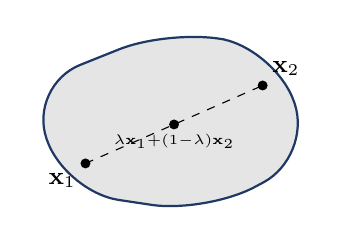
\begin{tikzpicture}[scale=0.9]
    \draw[fill=gray!20,draw=MainBlue,thick,rounded corners=20pt]
      (0,0) -- (2,-0.3) -- (3.5,0.5) -- (3,2) -- (1.5,2.3) -- (-0.5,1.5) -- cycle;
    \fill (0.3,0.4) circle (2pt) node[below left,font=\small]{$\bx_1$};
    \fill (2.8,1.5) circle (2pt) node[above right,font=\small]{$\bx_2$};
    \fill (1.55,0.95) circle (2pt) node[below,font=\tiny]{$\lambda\bx_1{+}(1{-}\lambda)\bx_2$};
    \draw[dashed](0.3,0.4)--(2.8,1.5);
  \end{tikzpicture}
  \end{center}
\end{frame}

\begin{frame}{Convex Functions}
  \begin{block}{Definition}
    $f:\Real^d\to\Real$ is \textbf{convex} if for all $\bx_1,\bx_2$ and $\lambda\in(0,1)$:
    \[
      f(\lambda\bx_1+(1-\lambda)\bx_2) \;\leq\; \lambda f(\bx_1)+(1-\lambda)f(\bx_2)
    \]
    It is \textbf{strictly convex} if the inequality is strict for $\bx_1\neq\bx_2$.
  \end{block}
  \begin{itemize}
    \item Geometric view: the chord between any two graph points lies \emph{above} the graph.
  \end{itemize}
  \vspace{4pt}
  \begin{center}
  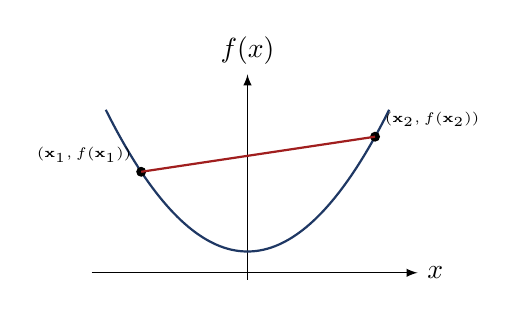
\begin{tikzpicture}[scale=0.9]
    \draw[->] (-2.2,0)--(2.4,0) node[right]{$x$};
    \draw[->] (0,-0.1)--(0,2.8) node[above]{$f(x)$};
    \draw[MainBlue,thick,domain=-2:2,samples=80] plot(\x,{\x*\x/2+0.3});
    \coordinate (P) at (-1.5,1.425);
    \coordinate (Q) at (1.8,1.92);
    \fill (P) circle(2pt); \fill (Q) circle(2pt);
    \draw[AlertRed,thick](P)--(Q);
    \node[font=\tiny,above left] at (P){$(\bx_1,f(\bx_1))$};
    \node[font=\tiny,above right] at (Q){$(\bx_2,f(\bx_2))$};
  \end{tikzpicture}
  \end{center}
\end{frame}

\begin{frame}{Why Convexity Matters}
  \begin{alertblock}{Key theorem}
    If $f$ is \textbf{convex}, any local minimum is also a \textbf{global minimum}.\\
    If $f$ is \textbf{strictly convex}, the global minimum is \textbf{unique}.
  \end{alertblock}
  \vspace{6pt}
  \begin{itemize}
    \item For a convex loss, solving $\nabla\calL(\bth;\calT)=\Zero$ \emph{guarantees} a global minimum.
    \item Gradient descent will converge to the optimum regardless of initialisation.
    \item \textbf{Sum rule}: a positively weighted sum of convex functions is convex.
    \item[$\Rightarrow$] if each $L(\bth;\bx_i,t_i)$ is convex, so is $\Rbar_{\calT}(h_{\bth})$.
  \end{itemize}
  \begin{block}{Practical implication}
    Designing convex loss functions makes optimisation reliable and predictable.
    Non-convex losses (e.g.\ in deep networks) require more sophisticated strategies.
  \end{block}
\end{frame}

\begin{frame}{Convexity in Practice}
  \begin{columns}[t]
    \column{0.46\textwidth}
      \begin{block}{Favourable cases}
        \begin{itemize}
          \item Linear regression $+$ quadratic loss: \emph{strictly convex}, closed-form solution.
          \item Logistic regression $+$ log loss: strictly convex.
          \item Linear SVM $+$ hinge loss: convex.
        \end{itemize}
      \end{block}
    \column{0.50\textwidth}
      \begin{alertblock}{Unfavourable cases}
        \begin{itemize}
          \item Deep neural networks: highly non-convex.
          \item Many saddle points; many local minima.
          \item Training requires careful initialisation and adaptive optimisers.
        \end{itemize}
      \end{alertblock}
  \end{columns}
  \vspace{6pt}
  \begin{itemize}
    \item When convexity cannot be guaranteed, use advanced methods:
          momentum, second-order approximations, learning-rate schedules, etc.
  \end{itemize}
\end{frame}

% =========================================================
\section{Common Loss Functions for Regression}
% =========================================================

\begin{frame}{Overview: Loss Functions for Regression}
  \begin{itemize}
    \item In regression, both $t$ and $h(\bx)$ are real-valued.
    \item Error $=$ some distance between prediction and target.
    \item Different distances $\Rightarrow$ different loss functions with different properties.
  \end{itemize}
  \vspace{8pt}
  \begin{center}
  \renewcommand{\arraystretch}{1.4}
  \begin{tabular}{lll}
    \toprule
    \textbf{Loss} & \textbf{Formula} & \textbf{Property}\\
    \midrule
    Quadratic (L2) & $(y-t)^2$ & Smooth, sensitive to outliers\\
    Absolute (L1)  & $|y-t|$   & Robust, non-smooth at 0\\
    Huber          & piecewise  & Best of both worlds\\
    \bottomrule
  \end{tabular}
  \end{center}
\end{frame}

% ----- Quadratic -----
\begin{frame}{Quadratic Loss (Squared Error)}
  \begin{block}{Definition}
    \[ L(y,t) = (y-t)^2 \]
  \end{block}
  \begin{itemize}
    \item Errors penalised \emph{quadratically}: doubling the error quadruples the loss.
    \item Empirical risk $\Rightarrow$ \textbf{Mean Squared Error (MSE)}:
      \[
        \Rbar_{\calT}(h)
        = \frac{1}{|\calT|}\sum_{(\bx,t)\in\calT}(h(\bx)-t)^2
      \]
    \item For linear regression $h(\bx)=\bw^T\bx+b$:
      \begin{itemize}
        \item Loss is \emph{strictly convex} in $(\bw,b)$.
        \item Gradient is linear $\Rightarrow$ closed-form solution (normal equations).
      \end{itemize}
    \item \textcolor{AlertRed}{Weakness}: very sensitive to outliers.
  \end{itemize}
\end{frame}

\begin{frame}{Quadratic Loss — Plot}
  \begin{center}
  \begin{tikzpicture}[scale=0.85]
    \draw[->](-2.8,0)--(2.8,0) node[right]{$y$};
    \draw[->](0,-0.2)--(0,3.5) node[above]{loss};
    \draw[MainBlue,thick,domain=-1.8:1.8,samples=80]
      plot(\x,{\x*\x}) node[right]{\small loss};
    \draw[AlertRed,dashed,domain=-1.8:1.8,samples=40]
      plot(\x,{2*\x}) node[right]{\small gradient};
    \node[font=\small] at (0,-0.4) {0};
  \end{tikzpicture}
  \end{center}
  \small Quadratic loss function and its gradient. Note the parabolic shape and the linear gradient.
\end{frame}

\begin{frame}{Quadratic Loss — Gradients for Linear Regression}
  For $h(\bx)=\bw^T\bx+b$, the gradients are:
  \[
    \frac{\partial}{\partial w_i}\calL
    = \sum_{(\bx,t)\in\calT}(\bw^T\bx+b-t)\,x_i
    \qquad
    \frac{\partial}{\partial b}\calL
    = \sum_{(\bx,t)\in\calT}(\bw^T\bx+b-t)
  \]
  \begin{itemize}
    \item Gradients are \emph{linear} in the parameters.
    \item Setting both to zero yields the \textbf{normal equations}.
    \item Exact, analytical solution — no iteration required.
  \end{itemize}
  \begin{alertblock}{Limitation}
    A single large outlier can dominate the sum and distort the entire fitted model.
  \end{alertblock}
\end{frame}

% ----- Absolute -----
\begin{frame}{Absolute Loss (L1)}
  \begin{block}{Definition}
    \[ L(y,t) = |y-t| \]
  \end{block}
  \begin{itemize}
    \item Errors penalised \emph{linearly}: doubling the error doubles the loss.
    \item Much more \textbf{robust to outliers} than quadratic loss.
    \item Gradient: piecewise constant, $\pm 1$ — steps of uniform size during GD.
    \item Convex but \emph{not} strictly convex; gradient undefined at $y=t$.
    \item Multiple optimal solutions possible; handled via \textbf{subgradient methods}.
  \end{itemize}
\end{frame}

\begin{frame}{Absolute Loss — Plot}
  \begin{center}
  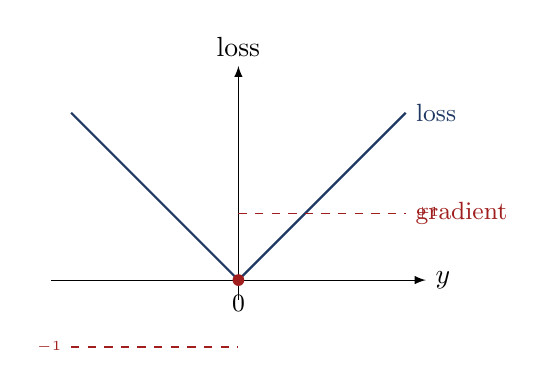
\begin{tikzpicture}[scale=0.85]
    \draw[->](-2.8,0)--(2.8,0) node[right]{$y$};
    \draw[->](0,-0.3)--(0,3.2) node[above]{loss};
    \draw[MainBlue,thick] (-2.5,2.5)--(0,0)--(2.5,2.5) node[right]{\small loss};
    \draw[AlertRed,dashed] (-2.5,-1)--(0,-1);
    \draw[AlertRed,dashed] (0,1)--(2.5,1) node[right]{\small gradient};
    \fill[AlertRed] (0,0) circle(2.5pt);
    \node[font=\small] at (0,-0.35) {0};
    \node[font=\tiny,left,AlertRed] at (-2.5,-1){$-1$};
    \node[font=\tiny,right,AlertRed] at (2.5,1){$+1$};
  \end{tikzpicture}
  \end{center}
  \small Absolute loss function and its gradient. The V-shape is characteristic, with constant gradient magnitude.
\end{frame}

% ----- Huber -----
\begin{frame}{Huber Loss}
  \begin{block}{Definition}
    \[
      L(t,y) = \begin{cases}
        \tfrac{1}{2}(t-y)^2 & |t-y|\leq\delta\\[4pt]
        \delta\!\left(|t-y|-\tfrac{\delta}{2}\right) & |t-y|>\delta
      \end{cases}
    \]
  \end{block}
  \begin{itemize}
    \item \textbf{Quadratic} for small errors $\Rightarrow$ smooth gradients, efficient optimisation.
    \item \textbf{Linear} for large errors $\Rightarrow$ robust to outliers.
    \item $\delta$ is a hyperparameter controlling the transition point.
    \item Combines the best properties of $L_2$ and $L_1$.
  \end{itemize}
\end{frame}

\begin{frame}{Huber Loss — Plot}
  \begin{center}
  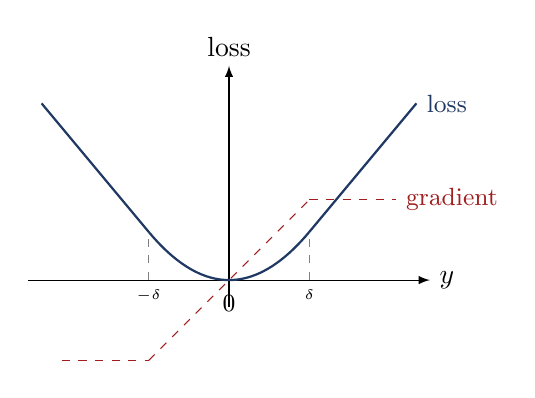
\begin{tikzpicture}[scale=0.85]
    \draw[->](-3,0)--(3,0) node[right]{$y$};
    \draw[->](0,-0.4)--(0,3.2) node[above]{loss};
    \def\del{1.2}
    % quadratic part
    \draw[MainBlue,thick,domain=-\del:\del,samples=40]
      plot(\x,{0.5*\x*\x});
    % linear parts
    \draw[MainBlue,thick]
      (-2.8,{abs(-2.8)*\del-0.5*\del*\del})--(-\del,{0.5*\del*\del});
    \draw[MainBlue,thick]
      (\del,{0.5*\del*\del})--(2.8,{abs(2.8)*\del-0.5*\del*\del})
      node[right]{\small loss};
    % gradient
    \draw[AlertRed,dashed,domain=-2.5:-\del,samples=5]
      plot(\x,-\del) node[left]{};
    \draw[AlertRed,dashed,domain=-\del:\del,samples=40]
      plot(\x,\x);
    \draw[AlertRed,dashed,domain=\del:2.5,samples=5]
      plot(\x,\del) node[right]{\small gradient};
    \draw[dashed,gray,thin](-\del,0)--(-\del,{0.5*\del*\del});
    \draw[dashed,gray,thin](\del,0)--(\del,{0.5*\del*\del});
    \node[below,font=\tiny] at (-\del,0){$-\delta$};
    \node[below,font=\tiny] at (\del,0){$\delta$};
    \node[font=\small] at (0,-0.35) {0};
  \end{tikzpicture}
  \end{center}
  \small Huber loss combines quadratic behaviour near zero with linear growth for large errors.
\end{frame}

\begin{frame}{Comparison: Regression Losses}
  \begin{center}
  \renewcommand{\arraystretch}{1.5}
  \begin{tabular}{lccc}
    \toprule
     & \textbf{L2} & \textbf{L1} & \textbf{Huber}\\
    \midrule
    Formula          & $(y-t)^2$       & $|y-t|$         & piecewise\\
    Convexity        & strictly convex & convex          & strictly convex\\
    Smoothness       & everywhere      & not at $y=t$    & everywhere\\
    Outlier robust   & low             & high            & high\\
    GD method        & direct          & subgradient     & direct\\
    Closed-form (linear) & \checkmark  & $\times$        & $\times$\\
    \bottomrule
  \end{tabular}
  \end{center}
\end{frame}

% =========================================================
\section{Loss Functions for Classification}
% =========================================================

\begin{frame}{Classification — Setup}
  \begin{itemize}
    \item Goal: assign inputs to \emph{discrete} classes.
    \item Focus on \textbf{binary classification}: $t\in\{-1,+1\}$.
    \item Classifier outputs a real value $y=h(\bx)$:
      \begin{itemize}
        \item $\mathrm{sign}(y)$ determines the predicted class.
        \item $|y|$ encodes prediction confidence.
      \end{itemize}
  \end{itemize}
  \vspace{6pt}
  \begin{columns}[t]
    \column{0.46\textwidth}
      \begin{block}{Direct prediction}
        Returns a class label $\hat t$.\\
        Error if $\hat t\neq t$.
      \end{block}
    \column{0.46\textwidth}
      \begin{block}{Probabilistic prediction}
        Returns $p(t|\bx)$ for each class.\\
        Error measured via distribution divergence.
      \end{block}
  \end{columns}
\end{frame}

% ----- 0/1 loss -----
\begin{frame}{0/1 Loss}
  \begin{block}{Definition}
    \[
      L(t,y) = \mathbb{1}[ty<0]
      \;\Leftrightarrow\;
      L(t,y) = \begin{cases} 1 & \mathrm{sgn}(y)\neq t\\ 0 & \mathrm{sgn}(y)=t \end{cases}
    \]
  \end{block}
  \begin{itemize}
    \item Directly minimises classification error rate. Intuitive.
    \item \textcolor{AlertRed}{Critical problems}:
      \begin{itemize}
        \item \textbf{Non-convex}: many local minima; no optimality guarantee.
        \item \textbf{Non-smooth}: discontinuous jump at $ty=0$.
        \item \textbf{Zero gradient almost everywhere}: gradient descent cannot progress.
        \item \textbf{NP-hard}: minimising $\overline{\mathcal{R}}$ for linear classifiers is computationally intractable.
      \end{itemize}
  \end{itemize}
\end{frame}

\begin{frame}{0/1 Loss — Plot}
  \begin{center}
  \begin{tikzpicture}[scale=0.9]
    \draw[->](-2.5,0)--(2.8,0) node[right]{$ty$};
    \draw[->](0,-0.3)--(0,1.8) node[above]{loss};
    \draw[MainBlue,very thick] (-2.5,1)--(0,1);
    \draw[MainBlue,very thick] (0,0)--(2.5,0);
    \fill[MainBlue](0,1) circle(3pt);
    \draw[MainBlue](0,0) circle(3pt);
    \node[font=\small] at (0,-0.4){$0$};
    \node[font=\small,left] at (0,1){$1$};
  \end{tikzpicture}
  \end{center}
  \small The 0/1 loss is a step function that assigns uniform cost to all errors.
\end{frame}

% ----- Surrogates -----
\begin{frame}{Convex Surrogate Loss Functions}
  \begin{block}{Motivation}
    0/1 loss is ideal but intractable. We replace it with a \textbf{surrogate} that is:
    \begin{enumerate}
      \item \textbf{Upper bound} on 0/1 loss: $L_{\mathrm{surr}}(t,y)\geq\mathbb{1}[ty<0]$
      \item \textbf{Convex} in $y$ (and in parameters).
      \item \textbf{Smooth}: well-defined derivatives almost everywhere.
    \end{enumerate}
  \end{block}
  \begin{block}{Key surrogates}
    Perceptron loss, Hinge loss, Log loss (cross-entropy), Squared loss (classification), Exponential loss.
  \end{block}
  \begin{itemize}
    \item Minimising a surrogate $\Rightarrow$ tends to minimise classification error indirectly.
  \end{itemize}
\end{frame}

% ----- Perceptron -----
\begin{frame}{Perceptron Loss}
  \begin{block}{Definition}
    \[ L(t,y) = \max(0,-ty) \]
  \end{block}
  \begin{itemize}
    \item \textbf{Correctly classified} ($ty>0$): loss $=0$. No penalty for correct predictions.
    \item \textbf{Misclassified} ($ty<0$): loss $=|ty|$. Severity grows with confidence of error.
    \item Continuous; gradient defined almost everywhere.
    \item Convex but \emph{not} strictly convex.
    \item \textcolor{AlertRed}{Not a proper surrogate}: does not always upper-bound 0/1 loss.
    \item Historical significance: underlies the classical \textbf{Perceptron algorithm} (1950s).
  \end{itemize}
\end{frame}

% ----- Hinge -----
\begin{frame}{Hinge Loss}
  \begin{block}{Definition}
    \[ L(t,y) = \max(0,1-ty) \]
  \end{block}
  \begin{itemize}
    \item Loss $=0$ only when $ty\geq 1$ (correct \emph{and} confident).
    \item $0<ty<1$: correct but not confident — still penalised.
    \item $ty<0$: misclassified — loss grows linearly.
    \item Properties: continuous, convex, proper surrogate (upper-bounds 0/1 loss).
    \item \textcolor{AlertRed}{Not differentiable} at $ty=1$ (corner); handled via \textbf{subgradients}.
    \item Foundation of \textbf{Support Vector Machines (SVM)}.
  \end{itemize}
\end{frame}

\begin{frame}{Hinge Loss — Plot}
  \begin{center}
  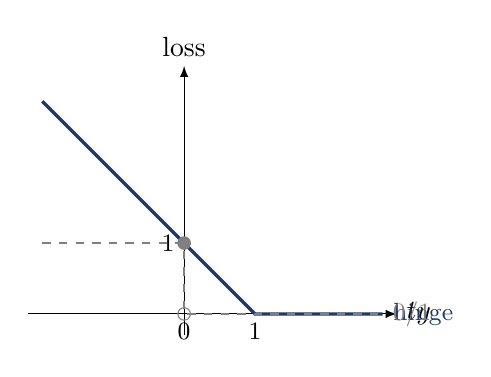
\begin{tikzpicture}[scale=0.9]
    \draw[->](-2.2,0)--(3,0) node[right]{$ty$};
    \draw[->](0,-0.3)--(0,3.5) node[above]{loss};
    % hinge
    \draw[MainBlue,very thick] (-2,3)--(1,0)--(2.8,0) node[right]{\small hinge};
    % 0/1
    \draw[gray,thick,dashed] (-2,1)--(0,1)--(0,0)--(2.8,0) node[right]{\small 0/1};
    \draw[gray,fill=gray](0,1) circle(2.5pt);
    \draw[gray](0,0) circle(2.5pt);
    \node[below,font=\small] at (0,0){$0$};
    \node[below,font=\small] at (1,0){$1$};
    \node[left,font=\small] at (0,1){$1$};
  \end{tikzpicture}
  \end{center}
\end{frame}

% =========================================================
\section{Subgradients}
% =========================================================

\begin{frame}{Non-Differentiable Losses — The Problem}
  Hinge loss: $L_H(t,y)=\max(0,1-ty)$
  \[
    \frac{\partial}{\partial y}L_H = \begin{cases}
      -t & ty<1\\ 0 & ty>1\\ \text{undefined} & ty=1
    \end{cases}
  \]
  \begin{itemize}
    \item The gradient is \textcolor{AlertRed}{undefined} at the corner $ty=1$.
    \item Standard gradient descent cannot be applied directly.
    \item Same issue arises for absolute loss at $y=t$ and perceptron loss at $ty=0$.
  \end{itemize}
  \begin{block}{Solution: subgradients}
    Generalise the gradient to non-smooth points using a \emph{set} of valid linear bounds.
  \end{block}
\end{frame}

\begin{frame}{Subgradients — Definition}
  For a convex function $f$, at a differentiable point $x$:
  \[
    f(x')\geq f(x)+\nabla f|_x\cdot(x'-x)\quad\forall x'
  \]
  (Gradient defines a tangent lower bound.)
  \begin{block}{Subgradient}
    A vector $\bar\nabla f|_x$ is a \textbf{subgradient} at $x$ if:
    \[
      f(x')\geq f(x)+\bar\nabla f|_x\cdot(x'-x)\quad\forall x'
    \]
  \end{block}
  \begin{itemize}
    \item At differentiable points: the subgradient is unique and equals the gradient.
    \item At non-differentiable points: there is a \emph{set} of valid subgradients.
    \item Any element of this set can be used in place of the gradient in GD.
  \end{itemize}
\end{frame}

\begin{frame}{Subgradient of Hinge Loss}
  At the corner $ty=1$, valid slopes lie between $-t$ and $0$.
  \vspace{8pt}
  \begin{center}
  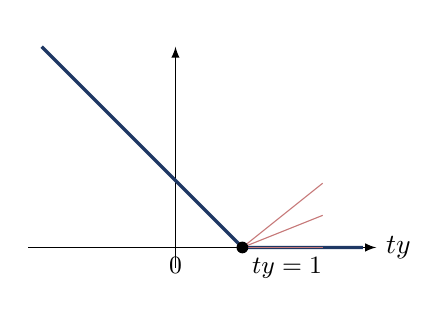
\begin{tikzpicture}[scale=0.85]
    \draw[->](-2.2,0)--(3,0) node[right]{$ty$};
    \draw[->](0,-0.3)--(0,3) node[above]{};
    \draw[MainBlue,very thick](-2,3)--(1,0)--(2.8,0);
    % subgradient fan
    \foreach \s in {-0.8,-0.4,0} {
      \draw[AlertRed!60,thin](1,0)--(2.2,{-\s*1.2});
    }
    \fill(1,0) circle(2.5pt) node[below right,font=\small]{$ty=1$};
    \node[below,font=\small] at (0,0){$0$};
    \node[below,font=\small] at (1,0){};
  \end{tikzpicture}
  \end{center}
  A common choice: set the subgradient to $0$ at $ty=1$, giving:
  \[
    \bar\nabla_y L_H = \begin{cases} -t & ty<1\\ 0 & ty\geq 1 \end{cases}
  \]
\end{frame}

% ----- Squared for classification -----
\begin{frame}{Squared Loss for Classification}
  \begin{block}{Definition}
    \[ L(t,y) = (1-ty)^2 \]
  \end{block}
  \begin{columns}[t]
    \column{0.46\textwidth}
      \begin{block}{Advantages}
        \begin{itemize}
          \item Infinitely differentiable.
          \item Convex, well-defined gradient.
          \item No corners or undefined points.
        \end{itemize}
      \end{block}
    \column{0.46\textwidth}
      \begin{alertblock}{Disadvantages}
        \begin{itemize}
          \item Not a proper surrogate: does not upper-bound 0/1 loss.
          \item Sensitive to outliers (quadratic growth).
          \item Penalises very confident correct predictions.
        \end{itemize}
      \end{alertblock}
  \end{columns}
  \vspace{4pt}
  \begin{itemize}
    \item Rarely the preferred choice in classification practice.
  \end{itemize}
\end{frame}

\begin{frame}{Squared Loss for Classification — Plot}
  \begin{center}
  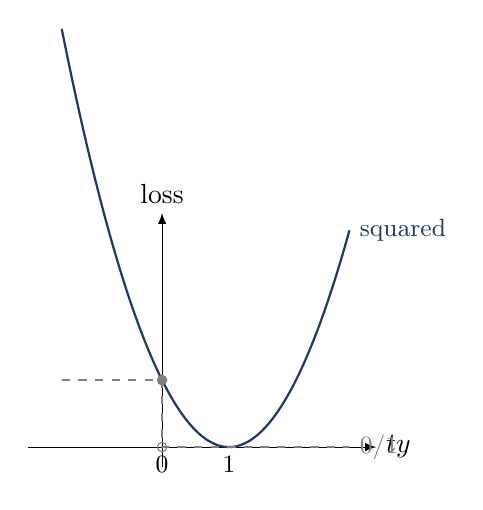
\begin{tikzpicture}[scale=0.85]
    \draw[->](-2,0)--(3.2,0) node[right]{$ty$};
    \draw[->](0,-0.3)--(0,3.5) node[above]{loss};
    % squared
    \draw[MainBlue,thick,domain=-1.5:2.8,samples=80]
      plot(\x,{(1-\x)^2}) node[right]{\small squared};
    % 0/1
    \draw[gray,dashed,thick](-1.5,1)--(0,1)--(0,0)--(2.8,0) node[right]{\small 0/1};
    \draw[gray,fill=gray](0,1) circle(2pt);
    \draw[gray](0,0) circle(2pt);
    \node[below,font=\small] at (0,0){$0$};
    \node[below,font=\small] at (1,0){$1$};
  \end{tikzpicture}
  \end{center}
\end{frame}

% =========================================================
\section{Log Loss and Information Theory}
% =========================================================

\begin{frame}{Log Loss (Cross-Entropy Loss)}
  \begin{block}{Definition}
    \[
      L(t,y) = \frac{1}{\log 2}\log\!\left(1+e^{-ty}\right)
    \]
  \end{block}
  \begin{itemize}
    \item Also called \textbf{logistic loss} or \textbf{cross-entropy loss}.
    \item Standard loss for probabilistic classification and logistic regression.
    \item Smooth approximation to hinge loss (no corner).
    \item For large negative $ty$: grows approximately linearly.
    \item For large positive $ty$: approaches 0 asymptotically (never reaches it).
  \end{itemize}
\end{frame}

\begin{frame}{Log Loss — Properties}
  \begin{columns}[t]
    \column{0.46\textwidth}
      \begin{block}{Mathematical properties}
        \begin{itemize}
          \item Infinitely differentiable everywhere.
          \item \textbf{Strictly convex}: unique global minimum.
          \item Proper surrogate: upper-bounds 0/1 loss.
          \item Gradient continuous and well-defined.
        \end{itemize}
      \end{block}
    \column{0.46\textwidth}
      \begin{alertblock}{Caution}
        \begin{itemize}
          \item Grows unboundedly for $ty\to-\infty$.
          \item Sensitive to severely mislabelled examples.
          \item Growth is logarithmic, so more robust than squared loss.
        \end{itemize}
      \end{alertblock}
  \end{columns}
\end{frame}

\begin{frame}{Log Loss — Plot}
  \begin{center}
  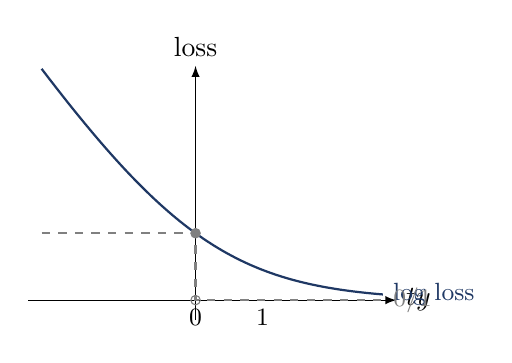
\begin{tikzpicture}[scale=0.85]
    \draw[->](-2.5,0)--(3,0) node[right]{$ty$};
    \draw[->](0,-0.3)--(0,3.5) node[above]{loss};
    % log loss
    \draw[MainBlue,thick,domain=-2.3:2.8,samples=80]
      plot(\x,{ln(1+exp(-\x))/ln(2)}) node[right]{\small log loss};
    % 0/1
    \draw[gray,dashed,thick](-2.3,1)--(0,1)--(0,0)--(2.8,0) node[right]{\small 0/1};
    \draw[gray,fill=gray](0,1) circle(2pt);
    \draw[gray](0,0) circle(2pt);
    \node[below,font=\small] at (0,0){$0$};
    \node[below,font=\small] at (1,0){$1$};
  \end{tikzpicture}
  \end{center}
\end{frame}

% ----- Info theory -----
\begin{frame}{Information Theory Background}
  \begin{columns}[t]
    \column{0.30\textwidth}
      \begin{block}{Entropy $H(p)$}
        \[ H(p)=-\mathbb{E}_{x\sim p}[\log p(x)] \]
        Uncertainty / information content of $p$.\\
        Min.\ avg.\ bits to encode from $p$.
      \end{block}
    \column{0.30\textwidth}
      \begin{block}{Cross-entropy $H(p,q)$}
        \[ H(p,q)=-\mathbb{E}_{x\sim p}[\log q(x)] \]
        Avg.\ bits using code for $q$, when true dist.\ is $p$.
      \end{block}
    \column{0.34\textwidth}
      \begin{block}{KL divergence}
        \[ \mathrm{KL}(p\|q)=H(p,q)-H(p) \]
        Extra bits wasted by using $q$ instead of $p$.\\
        Always $\geq 0$; $=0$ iff $p=q$.
      \end{block}
  \end{columns}
  \vspace{8pt}
  \begin{itemize}
    \item $\mathrm{KL}(p\|q)=0 \Leftrightarrow p=q$ (almost everywhere).
    \item Minimising cross-entropy $\equiv$ minimising KL divergence (since $H(p)$ is fixed).
  \end{itemize}
\end{frame}

\begin{frame}{Cross-Entropy for Binary Classification}
  Let $p(\bx)\in\{0,1\}$ be the true label, $y(\bx)\in[0,1]$ the predicted probability for class $C_1$.
  \begin{block}{Empirical cross-entropy}
    \[
      \mathrm{CE}(\calT)
      = -\frac{1}{|\calT|}
      \sum_{(\bx,t)\in\calT}\!
      \bigl[t\log y(\bx)+(1-t)\log(1-y(\bx))\bigr]
    \]
  \end{block}
  \begin{itemize}
    \item For each example: $\log$ probability assigned to the \emph{correct} class, averaged.
    \item The negative sign converts high probability (good) into low loss.
  \end{itemize}
  Separating by class:
  \[
    \mathrm{CE}(\calT)
    = -\frac{1}{|\calT|}
    \left(
      \sum_{(\bx,t)\in C_1}\!\log y(\bx)
      + \sum_{(\bx,t)\in C_0}\!\log(1-y(\bx))
    \right)
  \]
\end{frame}

\begin{frame}{Log Loss $\equiv$ Cross-Entropy (Logistic Regression)}
  For logistic regression:
  $y(\bx) = \sigma(\bw^T\bx+b) = \dfrac{1}{1+e^{-(\bw^T\bx+b)}}$
  \smallskip

  Substituting into cross-entropy, using $t\in\{-1,+1\}$:
  \[
    \mathrm{CE}(\calT)
    = \frac{1}{|\calT|}\sum_{(\bx,t)\in\calT}
      \log\!\left(1+e^{-t(\bw^T\bx+b)}\right)
  \]
  \begin{block}{Connection to log loss}
    \[
      \Rbar_{\calT}(h)
      = \frac{1}{|\calT|\log 2}
        \sum_{(\bx,t)\in\calT}
        \log\!\left(1+e^{-t(\bw^T\bx+b)}\right)
    \]
  \end{block}
  \begin{itemize}
    \item Minimising log loss $\equiv$ minimising cross-entropy.
    \item Strong information-theoretic justification for using log loss in classification.
  \end{itemize}
\end{frame}

% =========================================================
\section{Exponential Loss}
% =========================================================

\begin{frame}{Exponential Loss}
  \begin{block}{Definition}
    \[ L(t,y) = e^{-ty} \]
  \end{block}
  \begin{itemize}
    \item Prominent in \textbf{boosting} algorithms, especially \textbf{AdaBoost}.
    \item Penalises wrong predictions more aggressively than log loss: exponential growth.
    \item Infinitely differentiable everywhere.
    \item Strictly convex $\Rightarrow$ unique global minimum.
    \item Proper surrogate: upper-bounds 0/1 loss.
    \item \textcolor{AlertRed}{Sensitive to outliers}: very large penalty for confident misclassifications.
  \end{itemize}
\end{frame}

\begin{frame}{Exponential Loss — Plot}
  \begin{center}
  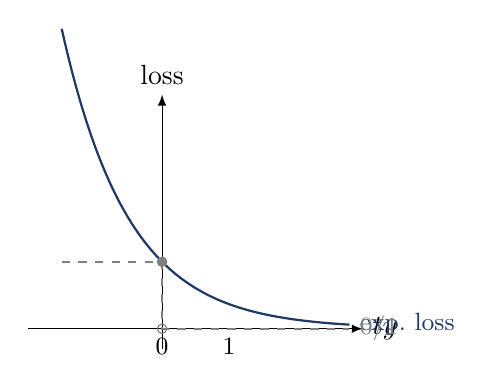
\begin{tikzpicture}[scale=0.85]
    \draw[->](-2,0)--(3,0) node[right]{$ty$};
    \draw[->](0,-0.3)--(0,3.5) node[above]{loss};
    % exp loss
    \draw[MainBlue,thick,domain=-1.5:2.8,samples=80]
      plot(\x,{exp(-\x)}) node[right]{\small exp.\ loss};
    % 0/1
    \draw[gray,dashed,thick](-1.5,1)--(0,1)--(0,0)--(2.8,0) node[right]{\small 0/1};
    \draw[gray,fill=gray](0,1) circle(2pt);
    \draw[gray](0,0) circle(2pt);
    \node[below,font=\small] at (0,0){$0$};
    \node[below,font=\small] at (1,0){$1$};
  \end{tikzpicture}
  \end{center}
\end{frame}

% ----- Classification comparison -----
\begin{frame}{Comparison: Classification Losses}
  \begin{center}
  \renewcommand{\arraystretch}{1.4}
  \begin{tabular}{lccccc}
    \toprule
     & \textbf{0/1} & \textbf{Perceptron} & \textbf{Hinge} & \textbf{Log} & \textbf{Exp.}\\
    \midrule
    Upper-bounds 0/1  & —    & partial  & \checkmark & \checkmark & \checkmark\\
    Convex            & No   & Yes      & Yes        & Yes        & Yes\\
    Strictly convex   & No   & No       & No         & \checkmark & \checkmark\\
    Smooth            & No   & No       & No         & \checkmark & \checkmark\\
    Outlier robust    & —    & medium   & medium     & medium     & low\\
    Use case          & ideal & Perceptron & SVM     & Logistic   & AdaBoost\\
    \bottomrule
  \end{tabular}
  \end{center}
\end{frame}

% =========================================================
\section{Summary}
% =========================================================

\begin{frame}{Summary — Loss Functions}
  \begin{block}{Core definitions}
    \begin{itemize}
      \item \textbf{Loss} $L(y,t)$: pointwise prediction penalty.
      \item \textbf{Empirical risk} $\Rbar_{\calT}(h)$: average loss over training set.
      \item \textbf{Training} $\equiv$ minimising $\Rbar_{\calT}(h_{\bth})$ over parameters $\bth$.
    \end{itemize}
  \end{block}
  \begin{block}{Regression losses}
    \begin{itemize}
      \item Quadratic (L2): smooth, convex, sensitive to outliers.
      \item Absolute (L1): robust, requires subgradients.
      \item Huber: best of both; controlled by $\delta$.
    \end{itemize}
  \end{block}
  \begin{block}{Classification losses}
    \begin{itemize}
      \item 0/1: intuitive but NP-hard to optimise.
      \item Surrogates (Hinge, Log, Exponential): convex, tractable.
      \item Log loss $\equiv$ cross-entropy: information-theoretic grounding.
    \end{itemize}
  \end{block}
\end{frame}

\begin{frame}{Summary — Optimisation}
  \begin{block}{Gradient descent}
    \begin{itemize}
      \item Iteratively follow the negative gradient.
      \item Learning rate $\eta$ controls step size.
      \item Converges to a local minimum (global if loss is convex).
    \end{itemize}
  \end{block}
  \begin{block}{Convexity}
    \begin{itemize}
      \item Convex loss: every local minimum is global.
      \item Strictly convex: unique global minimum.
      \item Sum of convex functions is convex $\Rightarrow$ empirical risk inherits convexity.
    \end{itemize}
  \end{block}
  \begin{block}{Variants \& Advanced Methods}
    \begin{itemize}
      \item Mini-batch / SGD: practical for large-scale learning.
      \item Subgradients: extend GD to non-smooth losses.
      \item Momentum, NAG, Adagrad, RMSprop, Adadelta, Adam: modern practice.
      \item Second-order (Newton, L-BFGS): powerful but costly.
    \end{itemize}
  \end{block}
\end{frame}

\begin{frame}{Central Message}
  \begin{center}
    \Large
    The loss function encodes what ``good predictions'' means.
  \end{center}
  \vspace{10pt}
  \begin{itemize}
    \item Choosing the right loss is as important as choosing the model.
    \item \textbf{Regression}: prefer L2 for smooth data, L1/Huber for outliers.
    \item \textbf{Classification}: use convex surrogates; log loss has the strongest theoretical backing.
    \item \textbf{Optimisation}: exploit convexity when possible; use SGD variants in practice.
    \item The interplay of loss, optimiser, and model defines the entire learning procedure.
  \end{itemize}
\end{frame}


